\documentclass[12pt, english, NoHyper]{AE4010-template}
\usepackage[]{natbib}
% \usepackage[sorting=none, citestyle=numeric-comp, natbib=true]{biblatex}    % For numbered biblatex references
% \usepackage[citestyle=authoryear]{biblatex}      % For author year biblatex references
\usepackage{csquotes}
\usepackage{hyperref}


%% Uncomment the following three lines when using the biblatex package
% \bibliography{bibliography.bib}
% \addbibresource{bibliography.bib}
% \bibliography{apa}
%% Uncomment the following line when using the natbib package
\bibliographystyle{plainnat}





%% Define your title entries here
\title{Orbital ascent trajectory optimization using reinforcement learning}
\author{Aaron M. de Windt}
\yourstudynumber{4134249}
\yourmscprofile{Control and Simulations}
\yourmsctrack{Control and Operations}









%   ########################################################################
%               PLEASE COMPILE USING XELATEX FOR THE BEST RESULTS
%   ########################################################################









\begin{document}
\maketitle

\section*{Executive Summary}
Interest in researching possible use cases of Deep Reinforcement Learning techniques in spacecraft guidance and control has been increasing in the past few years. This thesis proposes using these techniques to reduce the computational requirements needed to compute large batches of orbital ascent trajectories during the design process of new launchers. A trajectory optimization tool using Particle Swarm Optimization is used as a baseline to assess the accuracy of the trained RL agent. Proximal Policy Optimization (PPO) is used as the basis for the agent, furthermore a replay buffer and supervised learning techniques are used to speedup the initialization process of the agent by using expert demonstrations generated using the previously developed trajectory optimization tool. In case the accuracy of the RL agent is insufficient, it is investigated whether the optimization process of the trajectory optimization tool can be sped up by generating initial guesses using the RL agent. Reducing the computational requirements for computing new optimal orbital ascent trajectories is beneficial when evaluating the performance of a launcher design, specially when analyzing the  sensitivity of design parameters or when incorporated into a Multidisciplinary Design Optimization (MDO) project.




\section{Introduction}
Thanks to advancements in technology and an increasingly widespread use of satellite services, demand for space access has been steadily rising the past decades. This growth in the satellite launch services market has lead to the development of new launchers by both government agencies and an emerging private sector. 

One often overlooked, but crucial step during the design process of any product is the performance evaluation of proposed designs. This is the process of determining a products ability to meet the design requirements. Too low of a performance, and the product will not be able to fullfil its purpose. To high of a performance and the product may be over engineered or inefficient.

In the case of a launcher the performance may be measured by how much payload mass it can bring to it's target range of orbits. In other words, in order to maximize the performance of a launcher, the propellant mass fraction of the upper stage needs to be reduced.

A successful orbital insertion requires the launcher to carefully follow an optimized trajectory. This trajectory has a massive effect on the maximum performance of the launcher, but unfortunately finding the optimal trajectory is not a trivial. This problem falls under what is known as optimal control, a class of problems where the goal is to design a controller that optimizes a performance measure of a dynamical system's behavior over time, \cite{sutton2018reinforcement, betts2010practical}. 

A commonly used class of methods to compute orbital ascent trajectories is trajectory optimization. This is a set of mathematical techniques used to find the desired behavior of a dynamic system by finding the inputs as a function of time, \cite{betts2010practical, kelly2017introduction}. Trajectory optimization can be split in two groups, indirect and direct methods.

Indirect methods are more commonly used when computing orbital ascent trajectories, \cite{von1992direct}, due to their higher accuracy, but some direct methods have also been proposed, \cite{roh2002trajectory, jamilnia2012simultaneous, coverstone1994optimal}. More recently heuristic optimization methods, such as Particle Swarm Optimization (PSO) or Genetic Algorithm (GA), have been proposed in order to circumvent the initialization issues associated with indirect methods, \cite{pontani2014simple, zheng2020ascent}.

Using any of these methods to compute orbital ascent trajectories is computationally intensive and only yields open loop solutions for one particular trajectory. This is not an issue when calculating the trajectory for a launch during normal operations, but it is during the design process of a launch vehicle. 

A fast method to get a large number of trajectories is desired during the design process in order to, for example perform a sensitivity analyses on the design parameters, incorporate the trajectory solver into a larger Multidisciplinary Design Optimization (MDO) project, or continuously evaluate and monitor the feasibility of a changing design. 

This thesis proposes the use of Reinforcement Learning (RL) as a method to compute closed-loop solutions for orbital ascent trajectory problems. With enough training an RL agent is able to learn to solve complex and non-linear problems. Thus the goal is to develop an RL agent that is able to compute optimal trajectories for a wide range of initial states and launcher configurations within a single simulation run.

Even if generating optimal trajectories using RL ends up being unfeasible, it may still be able generate close to optimal trajectories, which may either be acceptable during the preliminary design phase, as a component of an MDO project, or serve as an initial guess for a more refined optimization algorithm.

The use of RL in spacecraft guidance, navigation and control opens up the possibilities to solve future problems as space exploration becomes more prevalent. For example thanks to its abilities to generalize and adapt in real time, it may be used in situations that are difficult to forsee or too cumbersome to manually take into account, such as hovering and manoeuvering around the non-uniform, rotating gravitational field of an asteroid, \cite{gaudet2012robust, willis2016reinforcement}, or performing docking operations with non-cooperative target objects in cluttered environments, \cite{hovell2020deep, hovell2021deep, broida2019spacecraft}.





\section{State-of-the-art/Literature Review}
The fields of trajectory optimization and reinforcement learning are quite extensive. The books from \cite{betts2010practical} and \cite{sutton2018reinforcement} are good starting points into these topics. The following two sections give an overview on the latest developments in these fields and finally applications of RL in spacecraft guidance are discussed. 

\subsection{Trajectory optimization}
Despite its disadvantages, indirect trajectory optimization methods are widely used when computing space flight trajectories. The main reason is the low accuracy associated with direct methods. In practice when using direct methods the minimum functional value found can be expected to have an error of about one percent which can be a crucial part of the payload in a space flight mission. Increasing the finite-dimensional space doesn't necessarily yield better results, \cite{von1992direct}.

One such indirect method is the Sequential Gradient-Restoration Algorithm (SGRA). Developed during the years 1968-86 by \cite{miele1970sequential}, this method has been successfully applied to atmospheric flight ,\cite{miele1986optimal}, space flight ,\cite{miele1999optimaltransfers, miele2001optimaltrajectories} and flights at the interface between atmosphere and space ,\cite{miele1998optimal, miele1993nominal, miele2000feasibility, miele2001assessment}. 

Recently newer techniques make use of heuristic optimization methods. A problem inherent to the methods already discussed is that since these methods are based on local computations, they are sensitive the starting guess and do not always converge towards the global optimum. On the other hand heuristic methods are global techniques which can look for the global optimum within a larger portion of the state space. The main idea behind heuristic optimization methods is that the search is done in a stochastic manner instead of a deterministic manner, \cite{rao2009survey}. However the main disadvantage of heuristic methods is the lack of any convergence proof and the capability of yielding only near optimal solutions, \cite{pontani2014optimal}.

These disadvantages can be circumvented by combining indirect and heuristic methods. As an example \cite{PONTANI2014852, pontani2013ascent, pontani2014simple, pontani2014optimal}, propose a method for computing the optimal exoatmospheric trajectory using PSO. The proposed method starts by analytically deriving the necessary conditions for optimality just as with indirect methods, then PSO is used to numerically determine the state, control and adjoint variables. The use of a heuristic method significantly lessens the initialization issues while retaining the accuracy and measure of accuracy that come with indirect methods.

\subsection{Reinforcement Learning}
Deep Reinforcement Learning (DRL) is a class of RL methods where a Deep Neural Network (DNN) is used as the function approximator. It offers a way to handle continuous state spaces, mitigate against state-action space explosion and generalize prior experience to previously unseen state-action pairs, \cite{kiran2021deep}. DRL methods have been able to learn policies that can reach human-level control for high-dimensional state spaces, \cite{mnih2015human, silver2016mastering}. 

One of the key issues with RL is sample efficiency. Animals are usually able to learn new tasks with just a few attempts by using prior knowledge. RL methods require too many samples before a reasonable policy is learned. Several methods have been developed to circumvent this, \cite{kiran2021deep}.

Experience replay allows agents to use a replay buffer to remember and reuse experiences that where observed in the past, thus increases the sample efficiency. Alternatively methods such as Asynchronous Advantage Actor Critic (A3C) and Advantage Actor Critic (A2C) execute multiple agents in parallel in order to generate the required experiences, \cite{mnih2016asynchronous}. 

Another way to improve sample efficiency is by trying to apply the largest possible learning updates per experience sample without over stepping. Methods such as Trust Region Policy Optimization (TRPO) and Proximal Policy Optimization (PPO) allow for multiple updates to be performed per experienced sample, while limiting the amount of change within a certain trust region, thus limiting the risk of overstepping, \cite{schulman2015trust, schulman2017proximal}.

Learning from Demonstrations (LfD) where the agents are trained using demonstrations from experts have been shown to be quite effective, specially during the initialization process. For example AlphaGo, \cite{silver2016mastering}, initializes the policy network using supervised learning on data from recorded human experts. Subsequent self-play was then able to improve and eventually achieve super human performance.
% 
Another approach is that taken by \cite{hester2018deep} to develop Deep Q-learning from Demonstrations (DQfD). DQfD augments the RL agent with a prioritized replay buffer and supervised learning losses to make effective use of the expert demonstrations, while still allowing the agent to learn based on it's own experiences 

\subsection{Reinforcement Learning in spacecraft guidance}
Research into the use of RL in spacecraft guidance is relatively young. The main characteristics of RL that are of special interest in space guidance is the ability to generalize and autonomously adapt to unknown situations that are difficult to predict or too cumbersome to take into account. This is specially useful for deep space missions due to the unavoidable communication lags which make it difficult for remote human operators to make adjustments in fast changing situations.

As an example the research by \cite{gaudet2012robust} explores the use of RL as a control method for hovering in the non-uniform, rotating gravitational field commonly associated with asteroids. The ability to generalize resulted in robust agents that could accurately hover in environments that where unknown during the policy optimization process.

More recently \cite{hovell2020deep, hovell2021deep} and \cite{broida2019spacecraft} have been developing RL based control system for proximity operation guidance, such as during autonomous rendezvous and docking operations. These could be applied in situations such as in-orbit servicing, assembly, and debris capture, where the chaser spacecraft may be required to manoeuvre in the proximity of a potentially uncooperative target object while avoiding nearby obstacles in cluttered environments. 

\cite{gaudet2018deep} propose the use of a PPO RL agent for planetary powered decent and landing. Future space missions will require spacecraft to target specific locations on the surface. The aim of this research is to develop a landing system that can land within a few meters from its target landing site. The agent was trained on a 6-DOF Mars landing simulation, and results demonstrated that the goal to achieve pin-point accuracy was reached.

RL has also been successfully demonstrated to be a suitable tool for developing control systems for efficient orbital change manoeuvre with low-thrust spacecraft, including for interplanetary trajectories, \cite{kolosa2019reinforcement, zavoli2020reinforcement, miller2020low}.

\section{Research Question, Aim/Objectives and Sub-goals}
The following two subsections present the research questions and research objective that are to be answered and met during the main thesis.

\subsection{Research Question(s)}
The main research question for the thesis can be formulated as:

\begin{quote}
\textbf{Can Reinforcement Learning be used to reduce the computational requirements for computing large batches of optimal orbital ascent trajectories for a range of launcher designs?}
\end{quote}

With this question in mind several sub-questions can be formulated. What are the limitations of current trajectory optimization methods? And what properties of RL can be used to circumvent them? Can RL methods be developed that outperform current methods in metrics such as accuracy and computational requirements? Or is it more effective to combine RL with current methods to potentially take advantage of the benefits of both?

\subsection{Research Objective}
\noindent The main research objective of this thesis is:

\begin{quote}
“To develop a tool capable of computing large batches of orbital ascent trajectories for a wide range of initial conditions and launcher configurations, by takes advantage of Reinforcement Learning and investigate its effectiveness with respect to existing methods, using metrics such as the accuracy of the results and computational requirements.”
\end{quote}

The sub goals for this objective are to implement an existing trajectory optimization method from literature, design and implement a novel method that takes advantage of RL, verify the accuracy of the new method using the existing one and compare the computational requirements of both methods when computing large batches of trajectories. A further sub-goal may be to combine the existing method with the novel method to produce a new hybrid method that takes advantage of the benefits of both.

\section{Theoretical Content/Methodology}
This will require the development three main pieces of code. A simulation, a traditional trajectory optimization method and a novel approach using Reinforcement learning. These will be presented in the following section.


\subsection{Simulation}
The simulation is kept as simple as possible. Only a 2D, 3-DOF dynamics on a circle shaped celestial body is considered. Initial experiments will be done without atmosphere and the celestial body will be non-rotating. These simplifications may potentially be removed if methods show to be effective. The simulation itself can be verified by comparing simulation results with existing models such JSBSim or verification data such as ``Standard Check-Cases for Six-Degree-of-Freedom Flight Vehicle Simulations'' \cite{unknown}.

\subsection{Existing trajectory optimization}
The method described by \cite{pontani2014simple} will be implemented as close as possible and validated against the results given in the paper. The method also includes a second order technique to evaluate the accuracy of the results, thus allowing for further verification.

\subsection{Reinforcement learning based method}
PPO, \cite{schulman2017proximal}, will be used as the main basis for the RL agent. A replay buffer will be added to improve sample efficiency, \cite{kiran2021deep}. To speed up the initialization process, the existing trajectory optimization method will be used to generate expert demonstrations which can be used by the agent using the technique described by \cite{hester2018deep}.

\subsection{Hybrid method}
It is likely that the RL agent may not be able to equal the accuracy of the existing method. However one drawback of the existing method is that it can take a long time to process before it yields a single result. Thus the stochastic policy of the trained RL agent may be used to generate initial guesses for the PSO used by the existing method to speedup the process. These should be close to the global optimal, thus not only will it take less time to converge, it may also require less particles. Optionally, if the results of the RL agent are close enough to the global optimal, then the PSO may be replaced by a simpler and faster deterministic optimization method.


\section{Experimental Set-up}
All software will be developed in python 3 with optimizations using Numba, Cython and C++. RLlib will be used as the RL framework since it already includes implementations of the target algorithms that can be used as a basis, it already implements replay buffers, has distributed computing tools and is actively used, well maintained and documented by the open source community and industry. Tensorflow will be used to create and train the Deep Neural Networks for similar reasons.

The entire project will be containerized using docker to allow the use of the distributed computing tools available in RLlib and guarantee portability of the end product.


\section{Results, Outcome and Relevance}
Once the RL agent has been trained, the accuracy of the results are verified against the traditional method by comparing results for cases which the agent didn't experience during the training process. If the RL agent cannot achieve a comparable level of accuracy as the traditional method. Then the hybrid tool will be developed.

Following this, the performance of the developed tools is compared by estimating the computational requirements per trajectory, while taking into account the resources needed during the training process and while computing output trajectories. The computational requirements per computed trajectory of the traditional tool is expected to remain constant with the total number of computed trajectories. However for the RL based tools it is expected to decrease with increasing number of output trajectories, since most of the computational expense was paid during the initial training process.

The resulting metrics can then give an insight into the value of the methods during the development process of future launch vehicles.


\section{Project Planning and Gantt Chart}
The simulation was already developed during the preliminary thesis phase, thus the main thesis can start directly with the development of the traditional trajectory optimization tool. Following that, the development of the RL agent may start and the database of expert demonstrations can be filled up in parallel by an automated program calling the traditional method.

Once the bulk of the code for the agent has been written the training and debugging processes can start and the midterm review can happen sometime during that process. Once the agent is fully trained, the experiments can be conducted. Finally the results can be processed and the final documentation can be done during the last few weeks before the thesis defence.

The project should nominally take 7 months to complete. Figure~\ref{fig:gantt} shows an overview of the overall timeline.


\section{Conclusions}
In conclusion, literature suggests that Reinforcement Learning has potential use cases in spacecraft guidance and control systems. The goal of this thesis is to investigate the potential of using RL based methods to reduce the computational requirements when computing large batches of trajectories during the design process of new launch vehicles.

The newly developed method will be compared against a more traditional trajectory optimization technique to assess the achievable level of accuracy. A hybrid method combining both the traditional and novel methods will also be developed and compared.

Once the experiments are done, the resulting performance metrics should give an insight of the value of the novel methods during the design process of new launch vehicles. 

\section{References}

%% Use letters for the chapter numbers of the appendices. 
%% Note: when there are references in the appendices, the references should be placed below the appendices.
\appendix
%% Uncomment the following line when using the natbib package
\bibliography{../../library/library}

%% Uncomment the following line when using the biblatex package
% \printbibliography


\section{Gantt Chart}
\begin{figure}[t]
    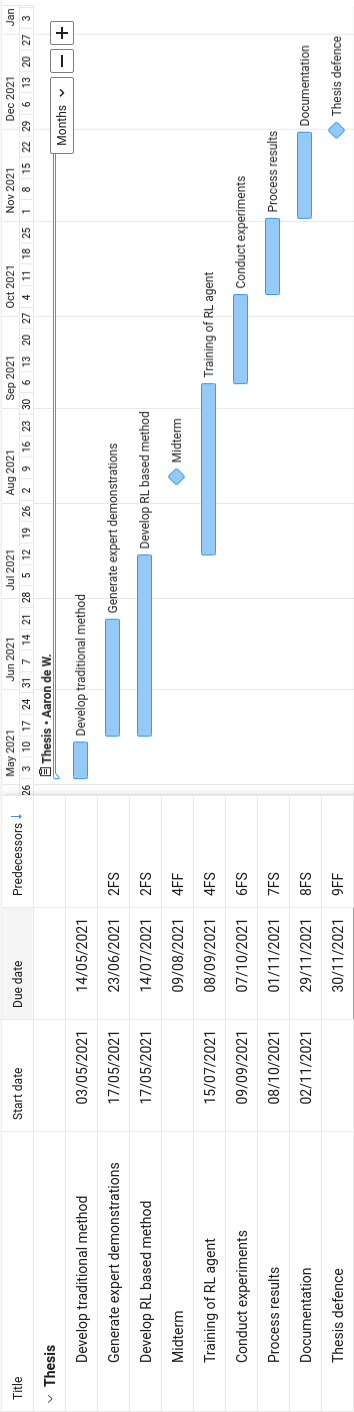
\includegraphics[width=6cm]{gantt}    
    \centering    
    \caption{Project timeline}
    \label{fig:gantt}
\end{figure}

\end{document}
